%\section{Runtime Architecture}

\subsection{Runtime}
\label{sec:runtime}

\begin{figure}
		\centering
		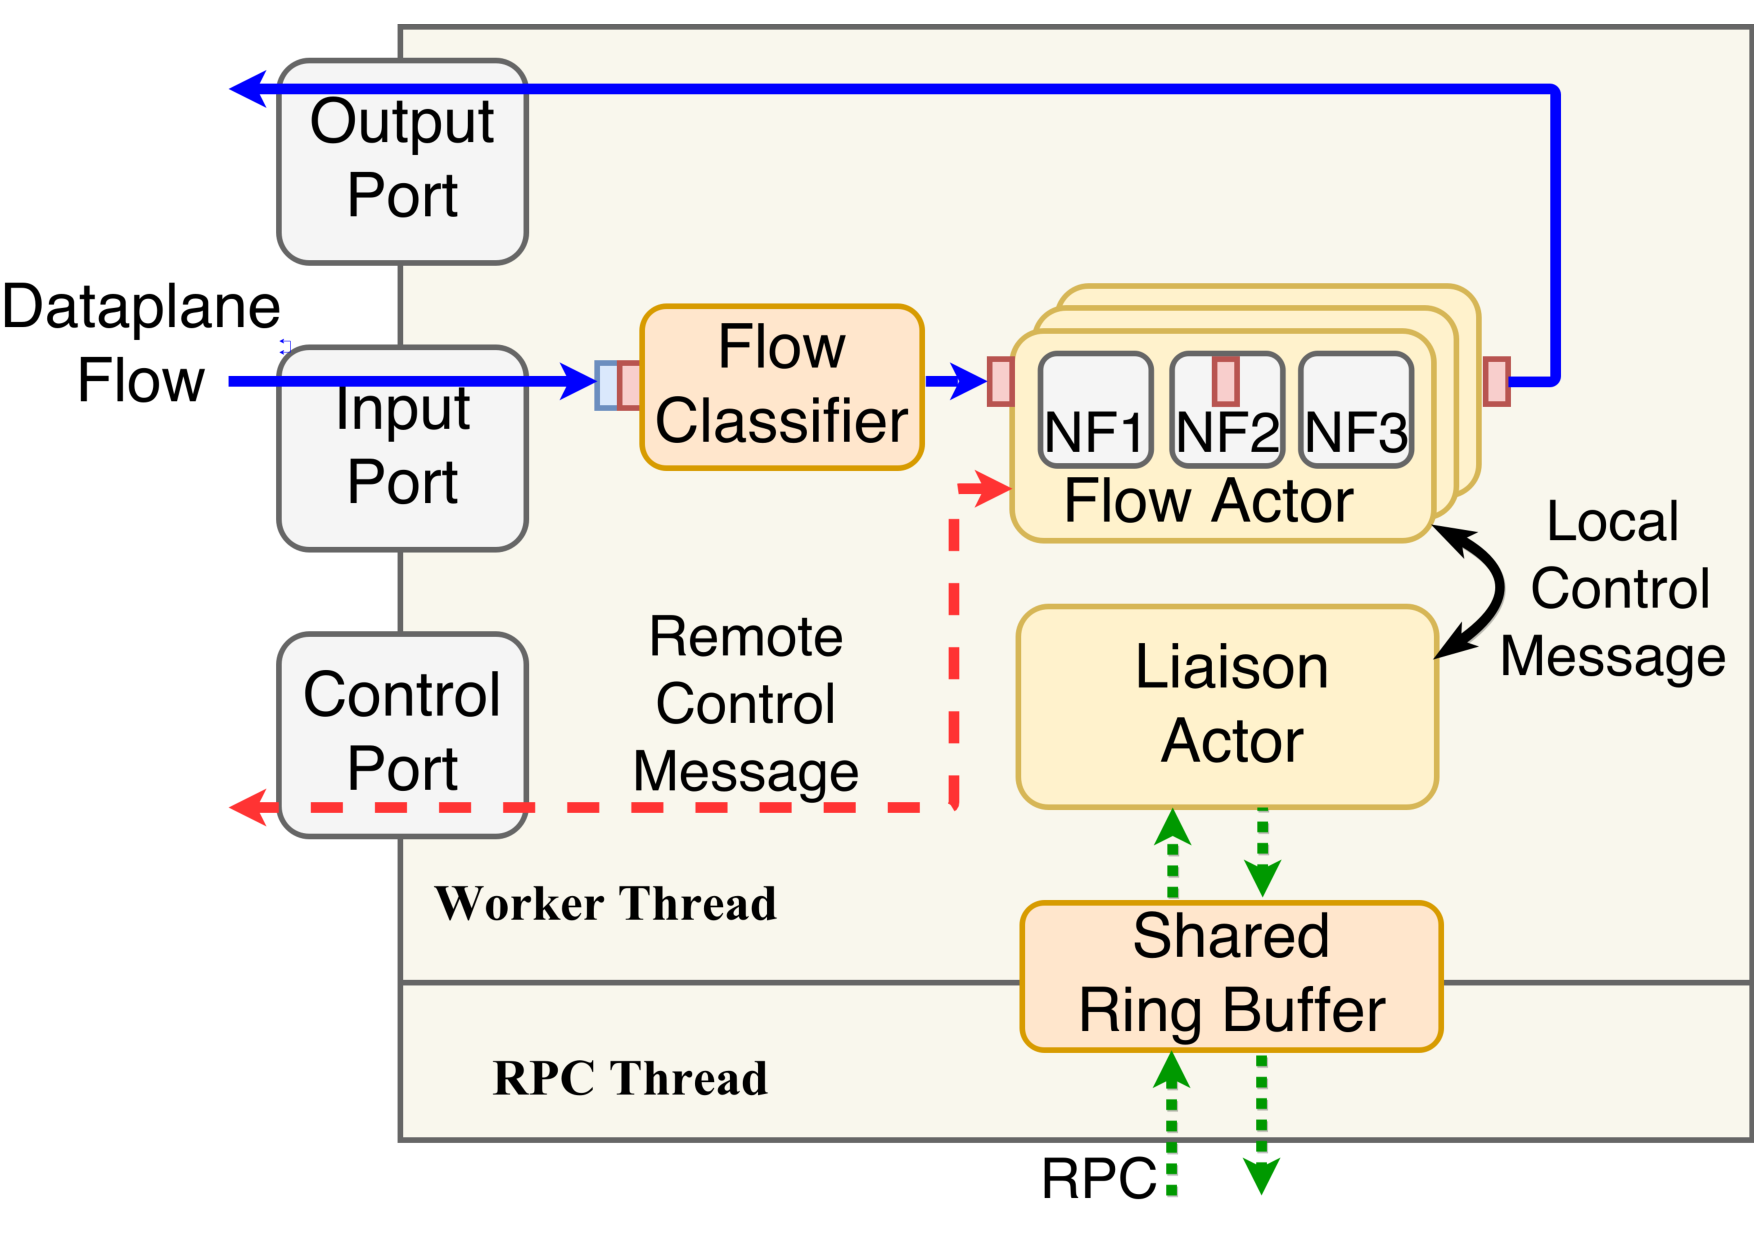
\includegraphics[width=\columnwidth]{figure/new-nfactor-runtime-arch.pdf}

		\caption{The internal structure of a runtime in \nfactor.}
\label{fig:runtime-arch}
\end{figure}

The concept of a uniform runtime system, as a basic flow processing and scaling unit in \nfactor, does not appear in most existing work \cite{bremler2015openbox, gember2012stratos, palkar2015e2}. In existing NFV systems, the basic flow processing and scaling unit is an NF instance, which is a virtual machine or container hosting an instance of a NF. % and the NF instances are chained on the data-plane. % The flows must go through these NF instances in sequence.
 The primary reason that we design such a runtime is to enable NFs/service chains to achieve failure resilience automatically without coordinator intervention, as the runtime provides a consistent communication channel
 %a network transparent abstraction \chuan{change this `network transparent' to a more accurate wording} to communicate and
 to exchange messages among each other, which are crucial for flow migration and replication.
  Especially, in a runtime, we adopt the simple yet powerful design to create a micro execution context for each flow, and encapsulate processing functions of the flow over its entire service chain inside the micro execution context. Then we can enable failure resilience on the basis of each micro execution context (Sec.~\ref{sec:resilience}). To be able to process multiple flows, the runtime is capable of handling multiple micro execution contexts concurrently.

In \nfactor, we exploit the actor programming model to implement the micro execution context. Each micro execution context is a flow actor. Flow processing by NFs in the service chain, flow migration and replication functionalities are all implemented as message handlers of the flow actor. The runtime provides the basic runtime environment for all the flow actors that it has created.


Fig.~\ref{fig:runtime-arch} shows the internal structure of a runtime. The input and output ports are used for receiving and sending flow packets from and to virtual switches. \ac{The control port as well as the input and output port are used for transmitting and receiving actor messages exchanged among different actors running on different runtimes for flow migration and replication, which are directly encapsulated inside L2 packets and sent/received using DPDK.} %Both input port and output port could be used transmit and send actor messages as well, for instance, during the second request-response in the flow migration and during flow recovery.
 Input packets of dataplane flows are first sent to a flow classifier, which uses the classical 5-tuple of a flow (\ie, source IP address, destination IP address, transport-layer protocol, source port and destination port) to identify packets belonging to the same flow. One flow actor is created for each new flow. The flow actor loads NFs of the service chain configured in the runtime. All packets of the same flow are sent to the same flow actor, which processes them in sequence by passing them through NFs in the service chain.

Each runtime is configured with a specific service chain by the coordinator during its booting phase. The runtime installs and initializes all the NFs as specified in the service chain upon booting. When a flow actor is created, it loads these NFs and uses a number of carefully defined NF APIs, as given in Table \ref{table:api} in Sec.~\ref{sec:NFAPIs}, to allocate new flow states and store them as internal actor state %\chuan{not clear what `allocate flow states' means. extract?}
and xxx \chuan{describe what it does to facilitate flow migration and replication by rewriting the idea of the following sentence: `Besides service chain processing, the flow actor also provides an execution context for distributed flow migration and replication, in response to certain messages (Sec.~\ref{sec:resilience})'}.


Each runtime can host one or multiple flow actors for flows passing through the same service chain that the runtime is configured with, depending on its resource availability and performance isolation requirements. In case of a multi-tenant NFV system, we can run actors processing flows of the same tenant on the same runtime, but those of different tenants on different runtimes, for better security and isolation. When multiple flow actors are concurrently running on one runtime, they are scheduled by a worker thread: \chuan{clearly describe how the flow actors are scheduled} whenever a message is received at the actor's mailbox, .... In addition, our design of the NF modules in the next section will show that passing packets to a NF for processing in a flow actor is essentially just a function call; only one copy of each NF software needs to be loaded in a runtime, while the flow actors can all make use of it. %An actor itself is a very lightweight one as millions of actors could be spawned in seconds \cite{chs-rapc-16}.



The runtime also consists of a RPC thread for receiving RPC requests from the controller (for flow migration, replication, etc.) and responding to them. The RPC thread and the worker thread share a ring buffer, used for relaying RPC requests received by the RPC thread to a liaison actor in the worker thread. We use a high-speed shared ring buffer to achieve fast inter-thread communication \chuan{add citation}. The liaison actor is responsible for coordinating with flow actors to execute the RPC requests from the controller. % flow actor initialization, flow migration and flow replication. %Flow actor and coordinator actor could directly exchanges local messages, or exchange remote messages through a reliable message passing module \cite{}.





\vspace{1mm}
\noindent {\bf Discussions on Runtime Design Choices.} The design of supporting only one service chain in one runtime significantly reduces the overhead of installing many NFs and avoids service chain selection in one runtime, for higher packet processing efficiency (speed) and management simplicity. Our one-actor-one-flow design is useful for facilitating fast flow migration (Sec.~\ref{sec:resilience}), which migrates a flow by migrating the actor that processes it \chuan{revise to more accurate description}. There are a few possible alternatives to our one-actor-one-flow design: (1) {\em One flow actor handles multiple flows.} It compromises the efficiency of flow migration, especially when multiple flows come from different virtual switch actors. In this case, the flow actor must synchronize the responses sent from different virtual switch actors \chuan{clarify what are `responses sent from different virtual switch actors' and why the flow actor needs to sync them}, adding overhead to flow migration process. (2) {\em One flow actor runs one NF}. Additional overhead is needed for chaining multiple flow actors to constitute a service chain, lowering packet processing speed. %Therefore, the one-flow-one-actor design achieves a sweet point in minimizing the actor processing overhead and improving the efficiency of flow migration protocol design.
Instead of using multiple worker threads in a runtime, the single-worker-thread design guarantees a sequential execution order of flow actors, thereby completely eliminating the need to protect message passing by locks \chuan{message passing among flow actors or what?}, and achieving higher efficiency.




%The alternative design to one-runtime-one-service-chain is to dynamically configure multiple service chains on a single runtime. Then due to the one-flow-one-actor design, we need to do an additional service chain selection, based on some pre-defined rules. This adds additional overhead to the flow actor processing and increases the complexity when managing the NFActor cluster, because the controller must populates the service chain rule dynamically to each runtime. With the one-runtime-on-service-chain design, if another service chain is needed, the system administrator could launch a new NFActor cluster and configure a different service chain to use.




%The runtime is designed as a single-worker-thread architecture to decrease the overhead of flow actors. A high speed NFV system may process millions of packets every second and migrates tens of thousands of flows. At such a high processing rate, message passing protected by shared lock in multi-threaded actor runtime system may incur a huge overhead and hurt the packet throughput.
%The runtime is configured with a specific service chain during the boot phase and initializes all the NF modules as specified in the service chain. When a flow actor is created, it loads these modules and uses the flow state allocation method \ref{table:api} to allocates all the
%To process flows across a service chain, during the initialization phase of the runtime, a service chain specifier is passed in to the runtime. The runtime then loads all the NF modules as indicated in the service chain specifier. When the flow classifier creates a new flow actor, the flow actor also loads these NF modules on the service chain and passes the input packet along the NF modules in sequence.

%The reason that the runtime is designed as a single-worker-thread program is because the multi-worker-thread design may not bring significant performance gain. In our initial prototype implementation, we use LIBCAF \cite{caf} library to construct flow actors. LIBCAF library creates multiple worker threads and schedules flow actors to run on these worker threads. Because LIBCAF completely conceals the internal interfaces of the worker threads, we have to create a dedicated polling thread to poll packet from the input port. Under this design, we find that the maximum throughput of a runtime does not increase when the number of LIBCAF worker thread increases, because the polling thread has always been a bottleneck. Therefore, we abandon the multi-worker-thread design and use a single worker thread to poll packets and schedule flow actors. To our surprise, this architecture turns out to work very well because it allows us to perform aggressive optimization of actor programming model \ref{}. In the mean time, we can still maintain the scalability of the system by launching more runtimes.

\subsection{NF APIs}
\label{sec:NFAPIs}

To achieve transparent resilience together with the micro execution environments provided by runtimes in \nfactor, an important step is to separate useful NF states from the core processing logic of each NF. With this separation, a flow actor can retrieve and serialize NF states for transmission whenever needed, without interfering with packet processing of the NF. In \nfactor, we achieve this separation by designing a set of APIs that NF implementation should follow in \nfactor.

\begin{table}[!t]
\centering
\caption{APIs to be Implemented by NFs in \nfactor.}
\label{table:api}
\resizebox{\columnwidth}{!}{
\begin{tabular}{c|l}
\textbf{API}                                      & \multicolumn{1}{c}{\textbf{Usage}}                                                                                                                                                                                                         \\ \hline
nf.allocate\_new\_fs()                            & \begin{tabular}[c]{@{}l@{}}Create a new flow state object for\\ a new flow actor, to be used for storing flow state\end{tabular}                                                                                                                                                  \\ \hline
nf.deallocate\_fs(fs)                             & \begin{tabular}[c]{@{}l@{}}Deallocate the flow state object\\ when the flow actor expires\\\end{tabular}                                                                                                                               \\ \hline
nf.process\_pkt(input\_pkt, fs)                   & \begin{tabular}[c]{@{}l@{}}Process the input packet using the \\ current flow state\end{tabular}                                                                                                         \\ \hline
%nf.get\_migration\_target(cluster\_cfg, fs) & \begin{tabular}[c]{@{}l@{}}Query an NF using the current\\ cluster configuration and \\ flow state about which runtime this flow\\ actor should be migrated to\end{tabular} \\ \hline
\end{tabular}
}
\end{table}


The APIs are given in Table \ref{table:api}, provided as four public methods for each NF to implement. When a new flow actor is created to handle a new flow, it first calls $nf.allocate\_new\_fs()$ to create a flow state object. Whenever the actor receives a new packet, the actor passes the received packet and the flow state object to \\
$nf.process\_pkt(input\_pkt, fs)$, for processing by the NFs, in sequence of the service chain. Any changes to the flow state when an NF has processed the packet is immediately visible to the flow actor. When the flow terminates, the flow actor expires and it calls $nf.deallocate\_fs(fs)$ to deallocate the flow state object. Using these three APIs, the flow actor always has direct access to the latest flow state, enabling it to transmit the flow state during flow migration and replication processes without disturbing packet processing of the NFs. %Therefore, the combination of the three methods servers as the basis for the transparent resilience in~\nfactor.

%\chuan{add the idea to flow migration section rather than exposign the API here} The fourth API $nf.get\_migration\_target(cluster\_cfg, fs)$ is used for checking where the NF would like the actor to migrate to, by passing the current cluster configuration and the current flow state. This enables the flow actor to actively migrate itself instead of waiting for migration initiation command sends from the controller \ref{}. This distributed design is the key to sparkle several useful applications, \ie, flow deduplication and reliable MPTCP subflow processing, which we will discuss in Sec.~\ref{sec:experiments}, that existing NFV systems based on centralized flow management cannot achieve. The flow actor should only call this method on the last NF in the service chain. Therefore NFs modules implementing this method should be placed on as the last NF in the service chain.

%These three methods are simple to use and properly generalize the structure of NFs that processes flow packets based on per-flow state. Using these three methods, we are able to create several representing NFs as shown in \ref{}.}

%The flow actor acquires the flow state of all the NF modules using the allocation API, and passes the packet across all the NF modules in sequence using the processing API.


To implement an NF in \nfactor, core processing logic of the NF needs to be implemented following the actor model and the APIs in Table \ref{table:api}. Nevertheless, porting the core
processing logic of an existing NF software is relatively straightforward. We have implemented a broad range of NFs in \nfactor and will present details in Sec.~\ref{sec:experiments}.


\subsection{Virtual Switch}
\label{sec:virtualswitch}

A virtual switch in \nfactor~is a special runtime where the actors do not run service chain but only a load balancer function. Following the one-actor-one-flow principle, a virtual switch can create multiple actors each to dispatch packets belonging to one flow.  We refer to the flow actor created by the virtual switch as virtual switch actor throughout this paper. Each switch receives information of the runtimes that it can dispatch flows to from the coordinator, including runtime's input port MAC addresses of the runtimes, load of the runtime, etc.


A virtual switch actor selects one of the available runtimes \chuan{define what available mean, not overloaded?} as its destination runtime in a round-robin way when it is created. We choose a simple round-robin algorithm because the vir- tual switch must run very fast and round-robin algorithm introduces the smallest amount of overhead while providing satisfactory performance. Whenever the virtual switch actor receives an input packet, it replaces the destination MAC address of the packet to destination runtime's input port MAC address, and modifies the source MAC address of the input packet to virtual switch's output port mac address. it then sends the packet out from the output port.


Virtual switch actors communicate with each other through remote control messaging \chuan{explain what this communication is used for in virtual switch}





Previous work either rely on SDN switches [20, 21] to route the traffic, or build a customized data-plane for inter- connecting different NF instances [31]. Our virtual switch is lightweight, only needs to dispatch flow to one runtime, but not individual NFs.


The architectural consistency of virtual switch and runtime facilitates flow migration and replication. The flow actor on the destination runtime could analyze the source MAC address of the packet and determine which virtual switch this packet comes from. This enables the flow actor to contact the virtual switch actor during flow migration and replication to change the destination runtime selected by the virtual switch actor \ref{}.

\subsection{Controller and Control RPCs}
\label{sec:controller}

To deploy a service chain in NFActor framework, the network administrator should first specify the configuration of the service chain to the controller and several SDN flow rules to match the input traffic. The controller then launches a new virtual switch and  a new runtime, configures the runtime with the service chain as required by the network administrator. Then the controller installs the SDN flow rules to direct the traffic to  virtual switch. Whenever the controller detects that the runtime connected with the virtual switch is overloaded, it scales up the cluster by launching a new runtime and configure the same service chain on that runtime.

The \nfactor's controller is responsible for monitoring the workload of each runtime and executing dynamic scaling. Due to the use of light-weight and distributed flow actors, the controller only needs to participate in the initiation phase of flow migration and replication. This feature differentiates \nfactor's controller with the controllers in OpenNF \cite{gember2015opennf} and Split/Merge \cite{rajagopalan2013split}, which need to fully coordinate the entire flow migration process. This simplifies the design of the controller and improve the failure resilience, as the controller does not need to maintain complicated states associated with flow migration.

Each runtime in NFActor regularly sends heartbeat messages to the controller, containing the current load information (i.e. CPU usage, memory usage) of the runtime. The controller gathers the information contained in the heartbeat messages into a cluster view list, which records the contact address, state (running, leaving, fail) and load information of all run- times. The controller broadcasts the cluster view list to each runtime and the virtual switch if there are any state/load changes, so that runtimes and virtual switch have a local copy of this list. The views at different runtime do not have to be consistent because flow migration and fault tolerance protocol perform safety checking by exchanging requests and responses to eliminate the inconsistency.

The controller manages \nfactor~using a series of control RPCs exposed by each runtime, which are summarized in Table \ref{table:rpc}. The controller uses PollWorkload RPC to acquire the current workload on a runtime and generates dynamic scaling decision. The controller maintains the configuration of the cluster, which include the mac address of input/output/control port and the ID of all the runtime and virtual switches. The controller notifies the cluster configuration to a runtime using NotifyClusterCfg RPC. The last three RPCs are used to initiate flow migration and replication. After issuing these three calls, migration and replication are automatically executed without further involving with the controller.

\chuan{briefly describe why using RPC}

assigns each runtime with a global unique ID to ease management.

\begin{table}[!h]
\centering
\caption{Control RPCs exposed from each runtime.}
\label{table:rpc}
\resizebox{\columnwidth}{!}{
\begin{tabular}{l|l}
Control RPC                                                                                   & Functionality                                                                                                                                              \\ \hline
PollWorkload()                                                                                   & \begin{tabular}[c]{@{}l@{}}Poll the workload information \\ from the runtime.\end{tabular}                                                                 \\ \hline
NotifyClusterCfg(cfg)                                                                         & \begin{tabular}[c]{@{}l@{}}Notify a runtime the current \\ cluster configuration.\end{tabular}                                                             \\ \hline
\begin{tabular}[c]{@{}l@{}}SetMigrationTarget(runtime\_id, \\ migration\_number)\end{tabular} & \begin{tabular}[c]{@{}l@{}}Initiate flow migration. It tells \\ the runtime to migrate \\ migration\_num flows to runtime\\ with runtime\_id.\end{tabular} \\ \hline
SetReplica(runtime\_id)                                                                       & \begin{tabular}[c]{@{}l@{}}Set the runtime with runtime\_id \\ as the replica.\end{tabular}                                                                \\ \hline
Recover(runtime\_id)                                                                          & \begin{tabular}[c]{@{}l@{}}Recover all the flows replicated \\ from runtime with runtime\_id.\end{tabular}                                                 \\ \hline
\end{tabular}
}
\end{table}

\section{Flow Management for Resilience}
\label{sec:resilience}

\subsection{Distributed Flow Migration}

\begin{figure}[!h]
\begin{subfigure}[t]{0.33\linewidth}
   \centering
   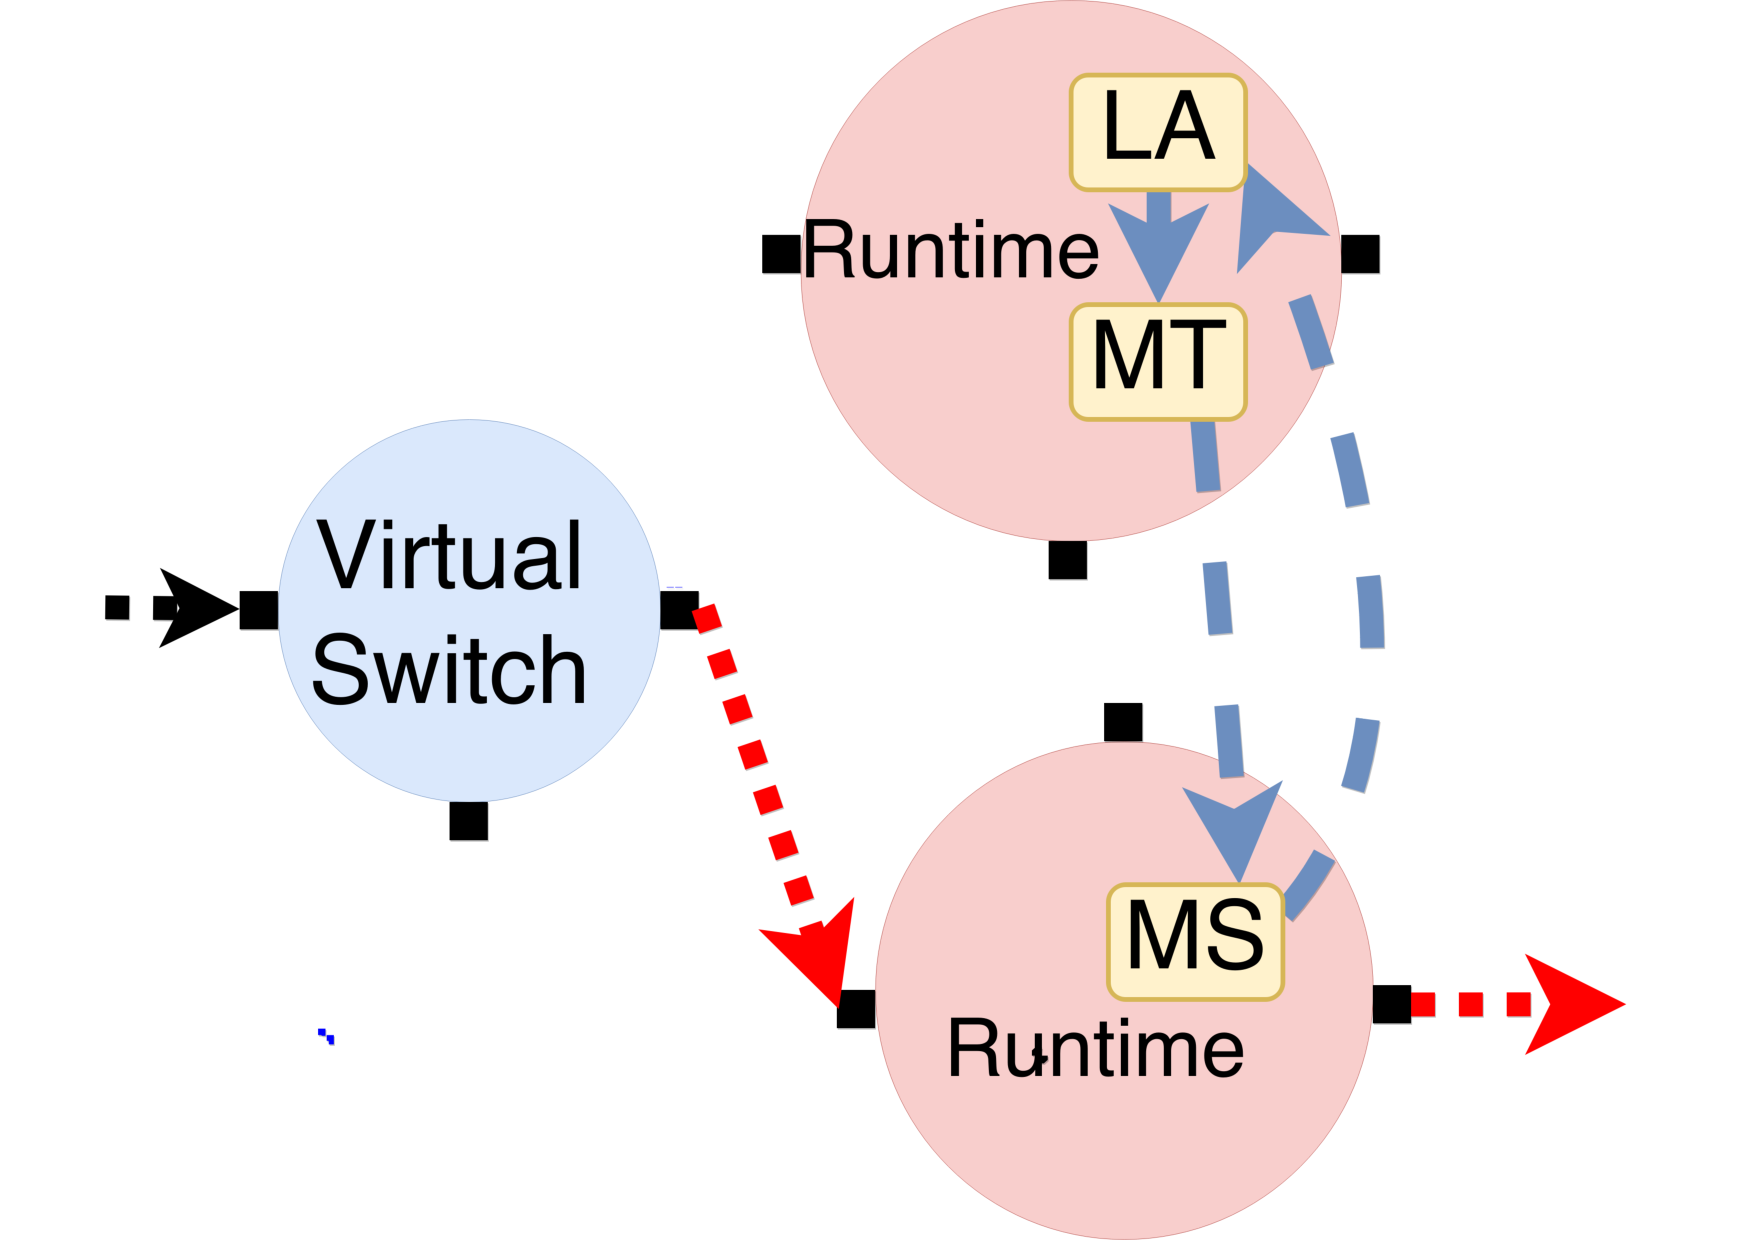
\includegraphics[width=\columnwidth]{figure/nfactor-mig1.pdf}
   \caption{1st req-rep.}\label{fig:mig1}
  \end{subfigure}\hfill
  \begin{subfigure}[t]{0.33\linewidth}
     \centering
     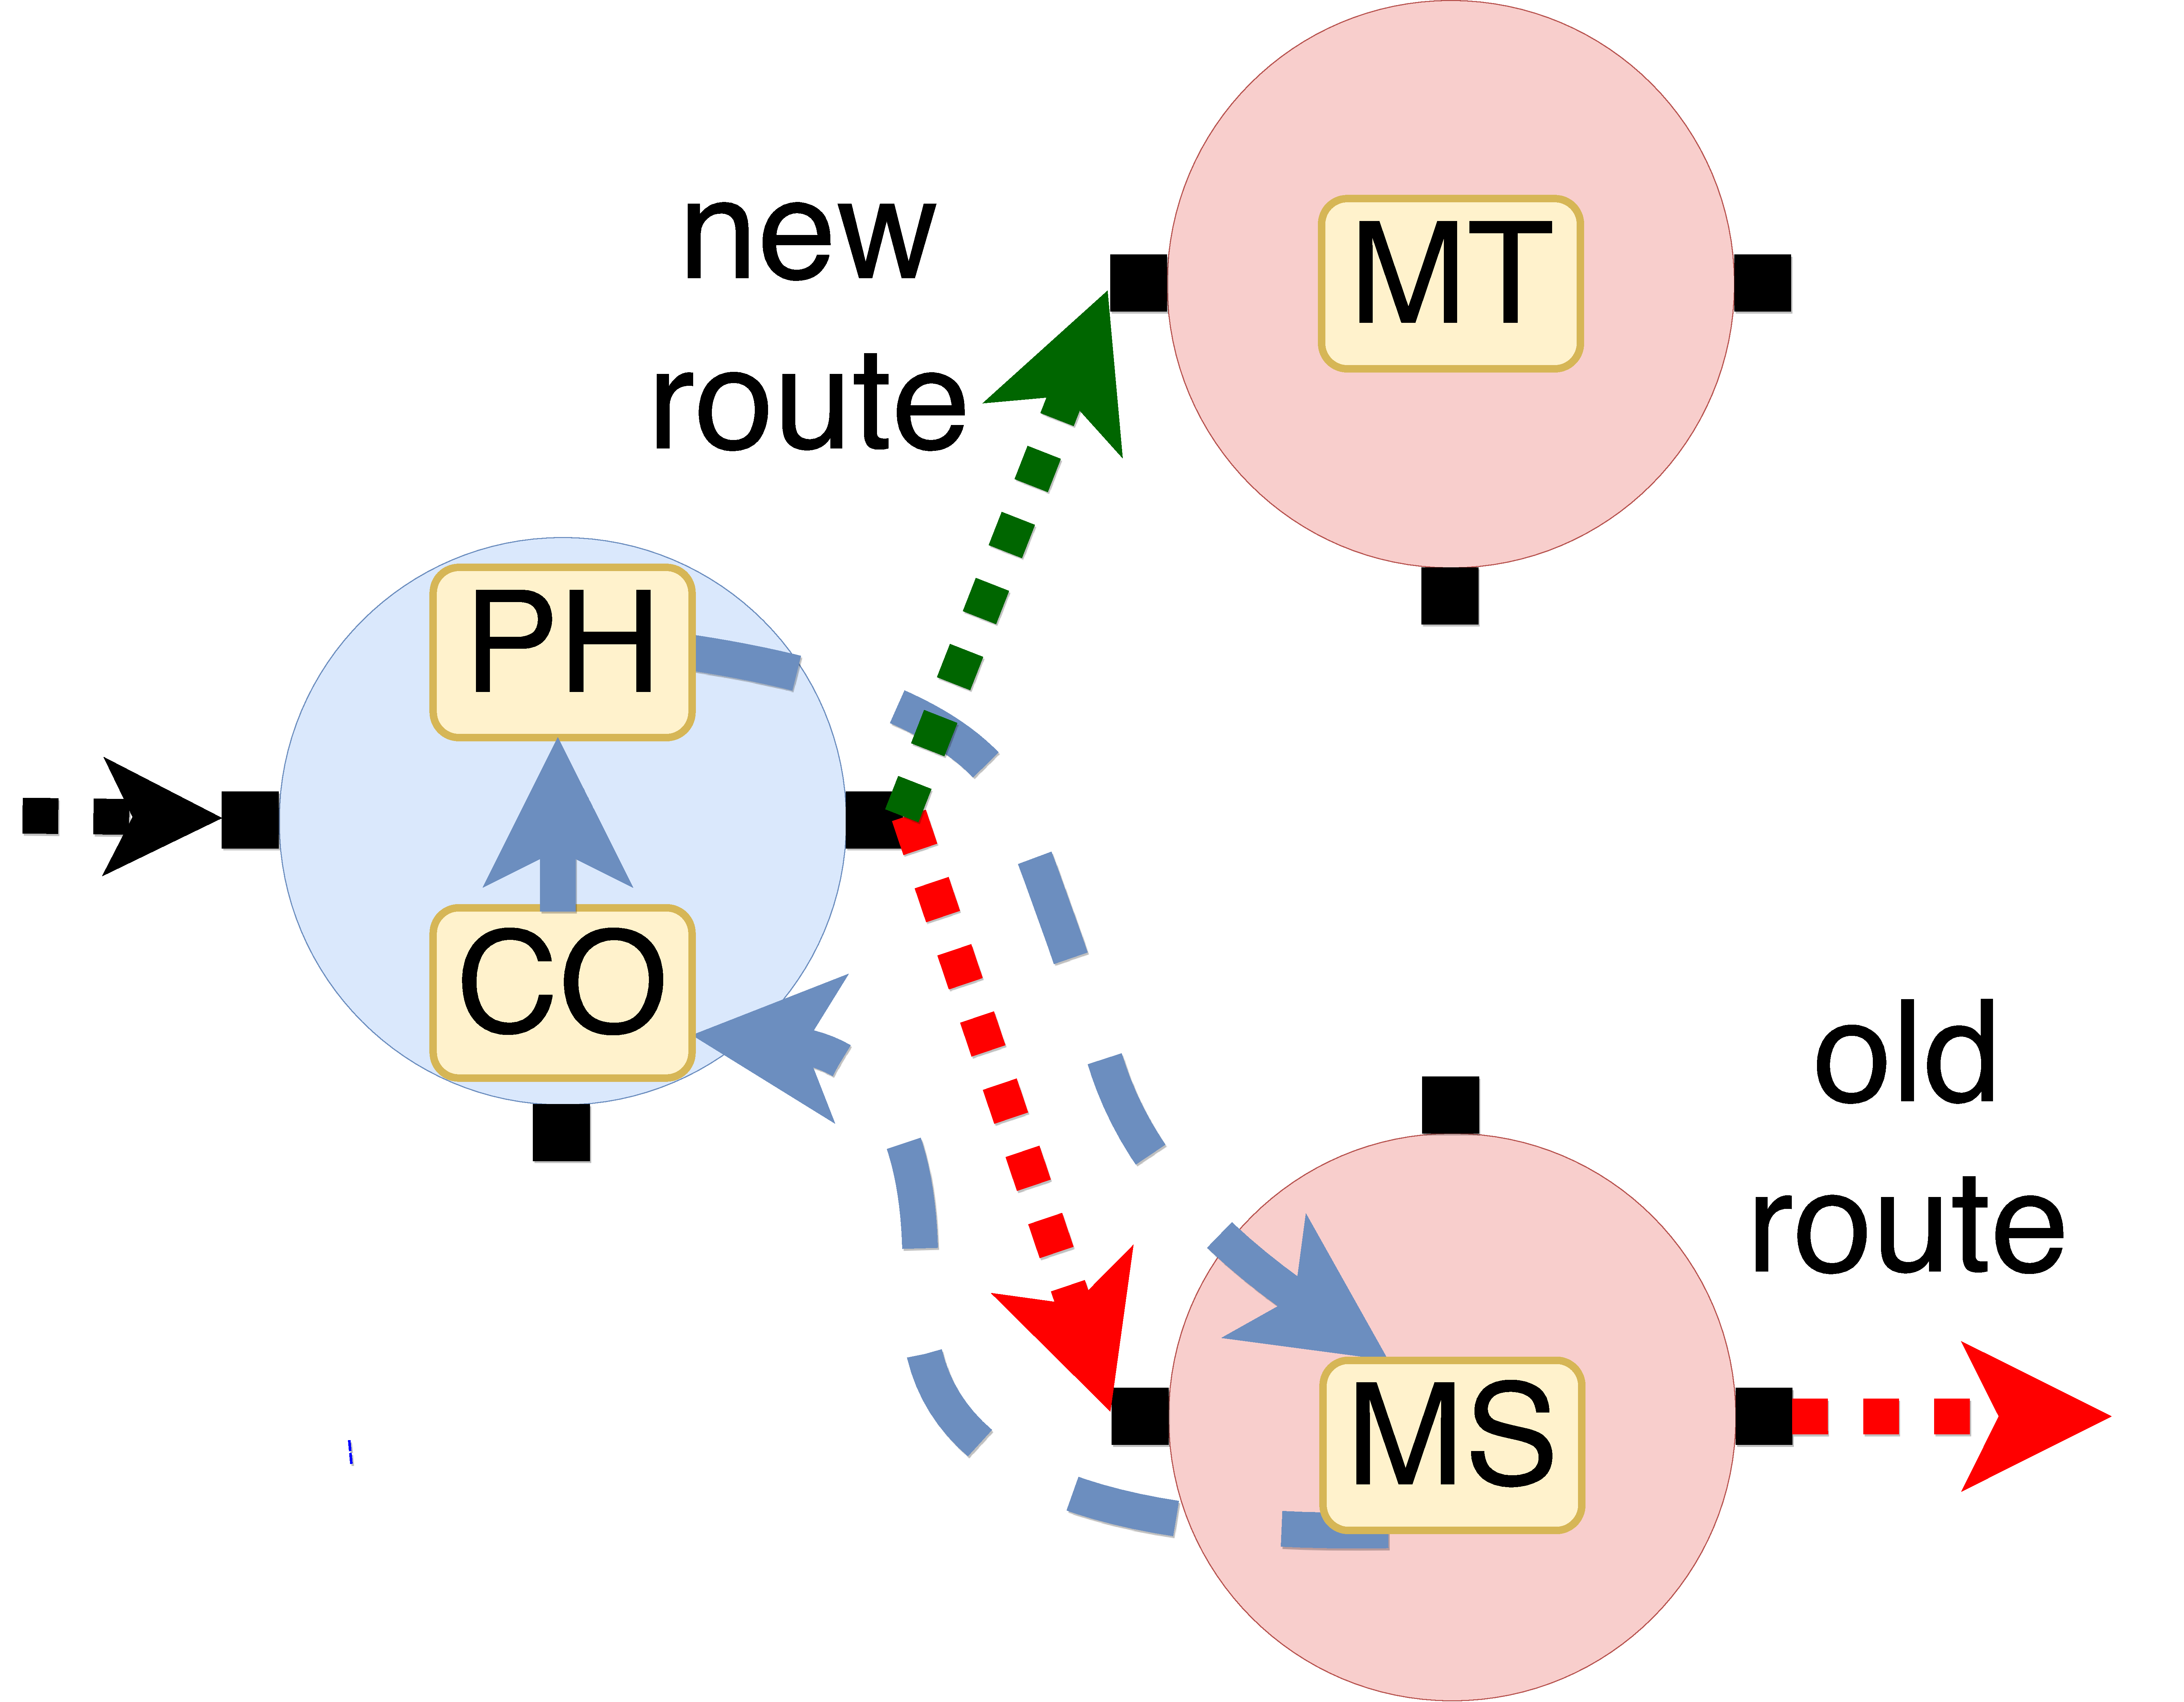
\includegraphics[width=\columnwidth]{figure/nfactor-mig2.pdf}
     \caption{2nd req-rep.}\label{fig:mig2}
    \end{subfigure}\hfill
  \begin{subfigure}[t]{0.33\linewidth}
 \centering
   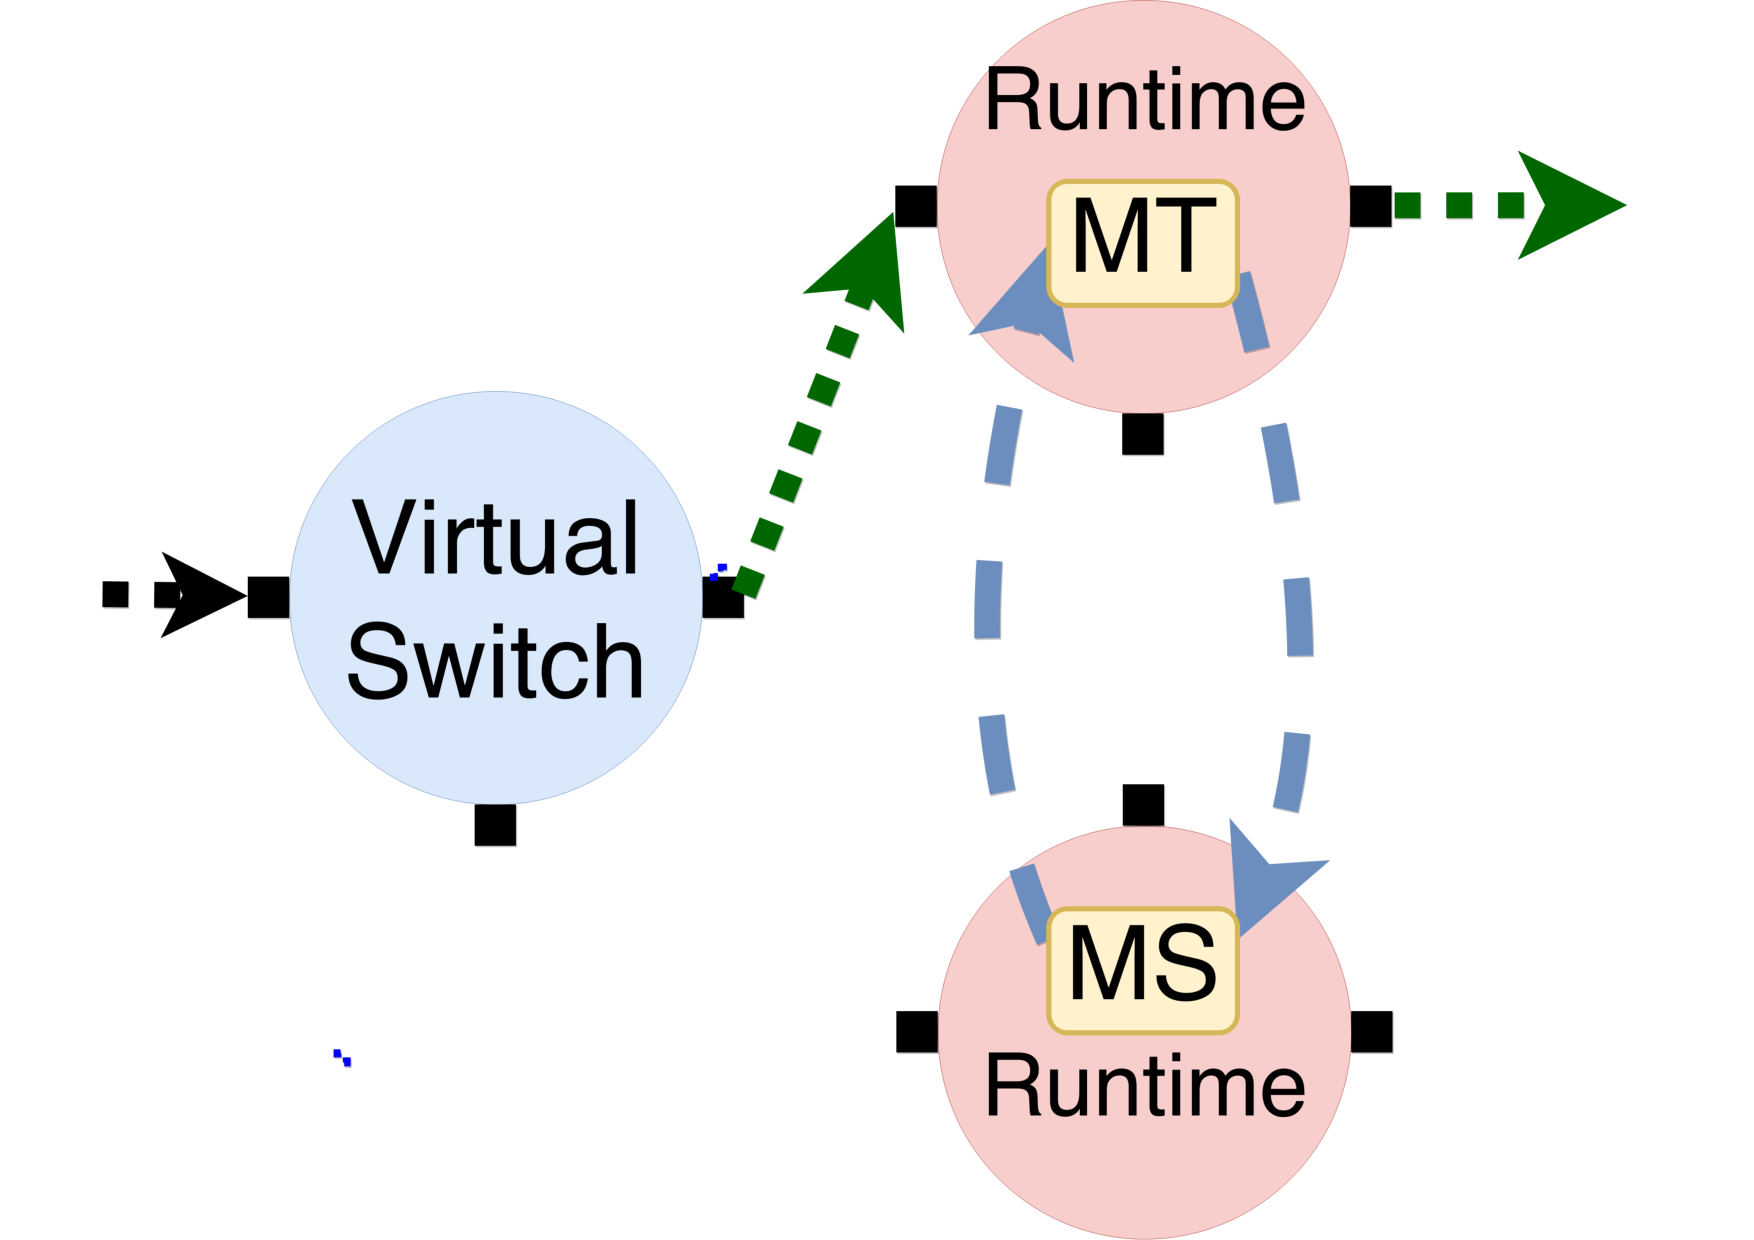
\includegraphics[width=\columnwidth]{figure/nfactor-mig3.pdf}
   \caption{3rd req-rep.}\label{fig:mig3} \end{subfigure}\hfill
 \caption{The flow migration process that migrates migration source actor running on migration source runtime to migration target runtime. (\textbf{MT}: Migration target actor. \textbf{MS}: Migration source actor. \textbf{CO}: Coordinator actor. \textbf{VS}: Virtual switch actor. \textbf{Dotted line}: Dataplane flow packets. \textbf{Dashed line}: Actor messages.)}
\label{fig:mig}
\end{figure}

Figure \ref{fig:mig} shows workflow of \nfactor's flow migration, which involves passing three request-response. Besides being fully distributed, the flow migration also guarantees two properties that (i) except for the migration target side buffer overflow or network packet reordering (which rarely happens in \nfactor), no flow packets are dropped by the flow migration protocol, which we refer to as \textbf{loss-avoidance} property (this is slightly weaker that the loss-free property in OpenNF \cite{gember2015opennf}) and (ii) the same \textbf{order-preserving} property as in OpenNF \cite{gember2015opennf}. There has been a long understanding that providing good properties for flow migration would compromise the performance of flow migration \cite{gember2015opennf}. \nfactor~ breaks this misunderstanding using the novel distributed flow migration.

Runtimes can check the received cluster view list to obtain the contact address and load information of other runtimes, and select an appropriate target for flow migration and repli- cation.

The details of the three request-responses are summarized below.
\begin{itemize}

\item \textbf{1st req-rep:} The migration source actor sends its flow-5-tuple to the coordinator actor on the migration target runtime. The coordinator actor creates a migration target actor using the flow-5-tuple contained in the request, which returns a response back to the migration source actor. During the execution of the first request-response, migration source actor continues to process packet.

\item \textbf{2nd req-rep:} The current flow actor sends its flow-5-tuple and the ID of the migration target runtime to the coordinator actor on the virtual switch. The coordinator actor uses the flow-5-tuple to find out the virtual switch actor and notifies it to change the destination runtime to migration target runtime. After changing the destination runtime, the virtual switch actor sends a response back to the migration source actor. The migration target actor starts to receive packets after the destination runtime of the virtual switch actor is changed and buffer all the received packets until it receives the third request. In the meantime, the migration source actor keeps processing the input packets until it receives the second response.

\item \textbf{3rd req-rep:} the migration source actor sends its flow state to the migration target actor. After receiving the flow states, the migration target actor saves them, gives a response to the migration source actor and immediately start processing all the buffered packets. The migration source actor exits when it receives the response.

\end{itemize}

\textbf{The Loss-Avoidance Property.} Before the migration target actor receives the third request, it needs to buffer input packets indefinitely, which might lead to a buffer overflow if the third request takes a long time to arrive. \nfactor~ simply drops additional flow packets after buffer overflow because \nfactor~ needs to process packet at a high throughput rate and does not want to grow buffer indifinitely. In \nfactor, a large collective buffer is used to buffer the packets for different migration target actors and the distributed flow migration process is extremely fast, so the buffer overflow rarely happens, even when migrating a huge number of flows. This is demonstrated in the evaluation section \ref{}.

Besides buffer overflow, the only step that might incur potential packet drop is in the third request-response. When the second response is received by the migration source actor, it must immediately send its flow state in the third request to the migration target actor. After sending the third request, there might be pending flow packets continuing to arrive at migration source actor. These pending packets are are sent out by the virtual switch actor before the destination runtime is changed. If this happens, the migration source actor has to discard these pending flow packets because it has already sent out the third request. Continuing to process these packets may generate inconsistent output packets.

If the network doesn't reorder packet, which is a common case because \nfactor~is deployed over a L2 network, \nfactor's flow migration can eliminate the second cause of packet drop by transmitting second response in a network packet over the same network path as the data plane packets that are sent to the migration source actor. Recall that in Figure \ref{fig:runtime-arch}, the remote messages could be sent over input/output port of a runtime. The second response is encapsulated in a raw packet \ref{}, sent by the output port of the virtual switch and received by the input port of the migration source runtime, therefore sharing the same network path as the data plane packets that are sent to the migration source actor.

Because the second response are sent after the destination runtime of the virtual switch actor is changed and share the same network path as the data plane packets that are sent to the migration source actor, it also becomes a strong indication that no more input packets will be sent to the migration source actor. This is verified in our evaluation \ref{}.

\textbf{Order-preserving Property.} Since the second request-response eliminate the packet drop if the network doesn't reorder packets, flow packets could always be processed in the order that they are sent out from the virtual switch. The order-preserving property is therefore guaranteed.

\textbf{Error Handling.} The three request-responses may not always be successfully executed. In case of request timeout, the migration source actor is responsible for restoring the destination runtime of the virtual switch actor (if it is changed) and resumes normal packet processing. The migration target actor is automatically deleted after a timeout.

\subsection{Scalable Flow Replication}

\begin{figure}[!h]
\begin{subfigure}[t]{0.49\linewidth}
   \centering
   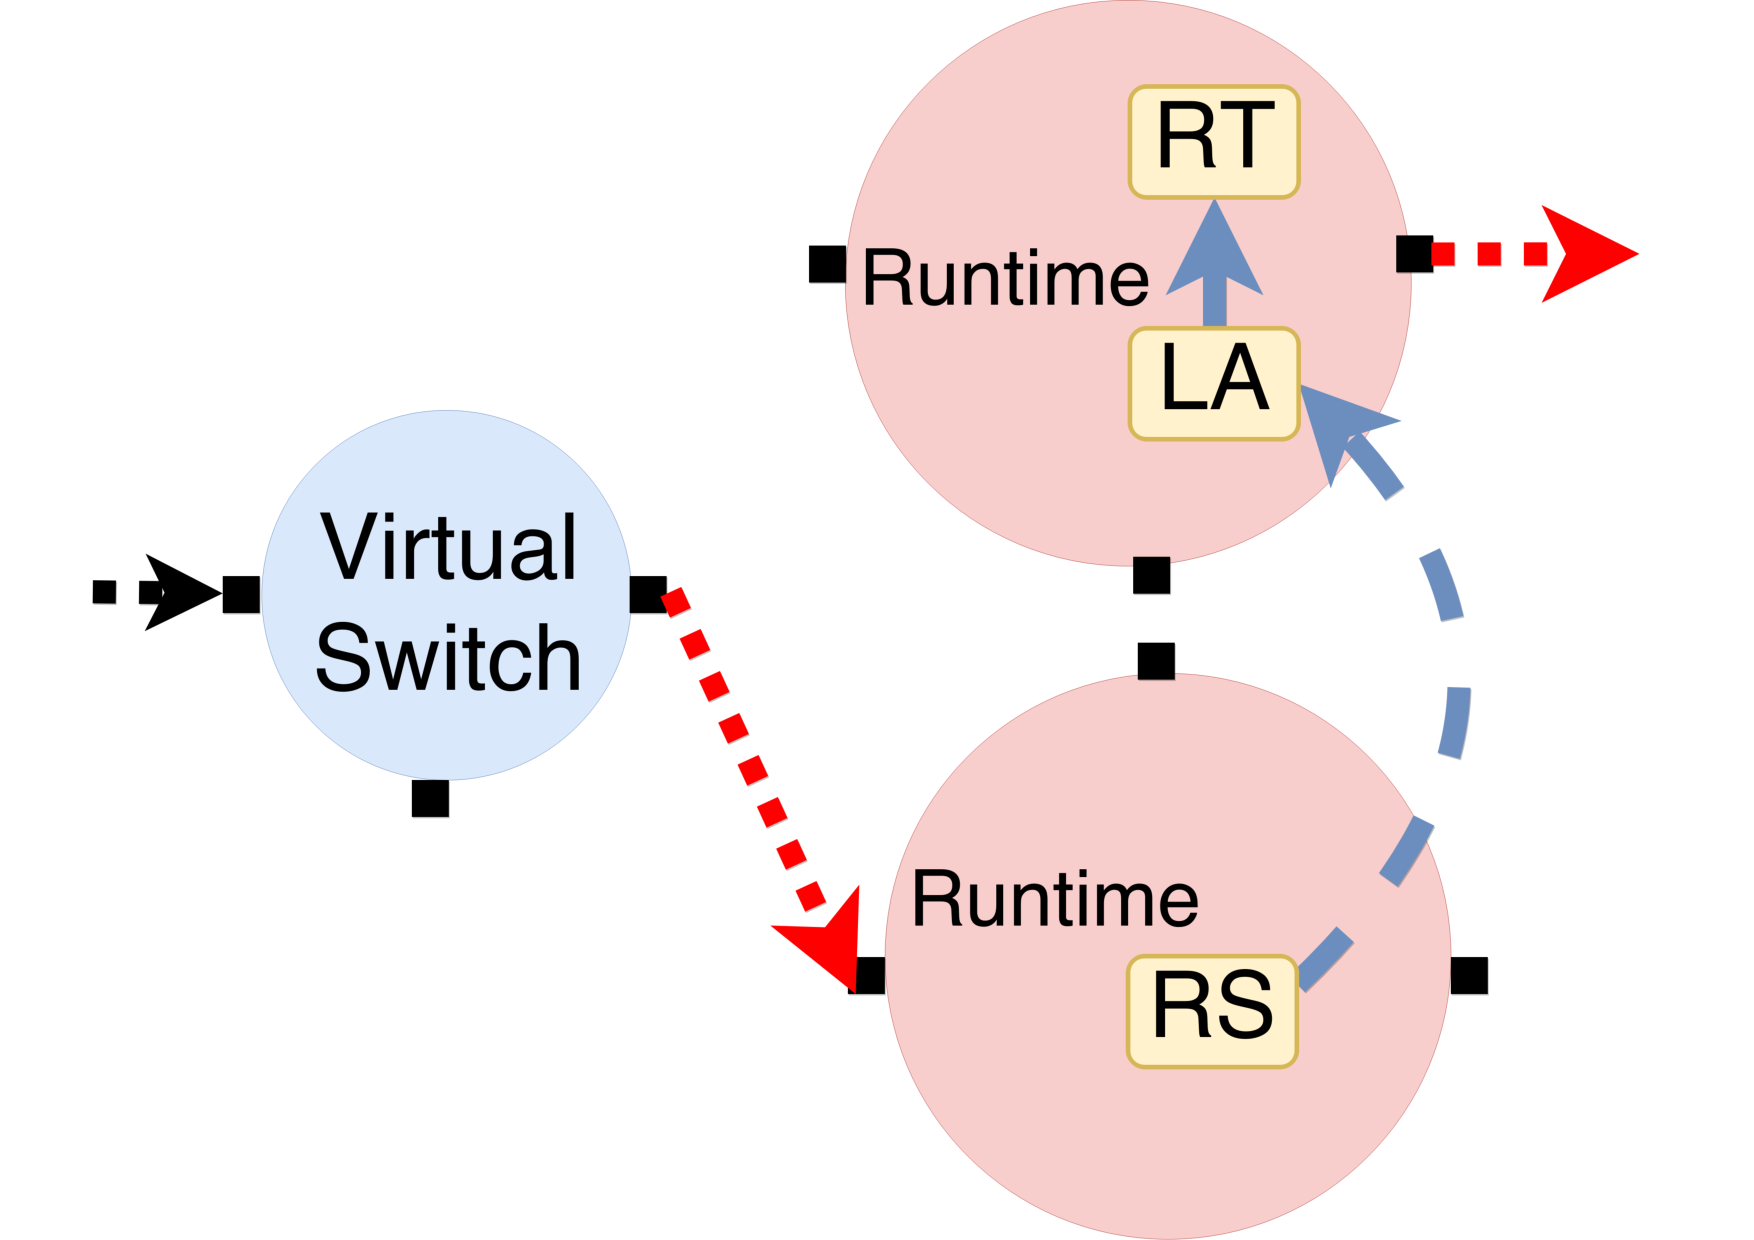
\includegraphics[width=0.66\columnwidth]{figure/nfactor-replication.pdf}
   \caption{Flow replication.}\label{fig:rep}
  \end{subfigure}
  \begin{subfigure}[t]{0.49\linewidth}
     \centering
     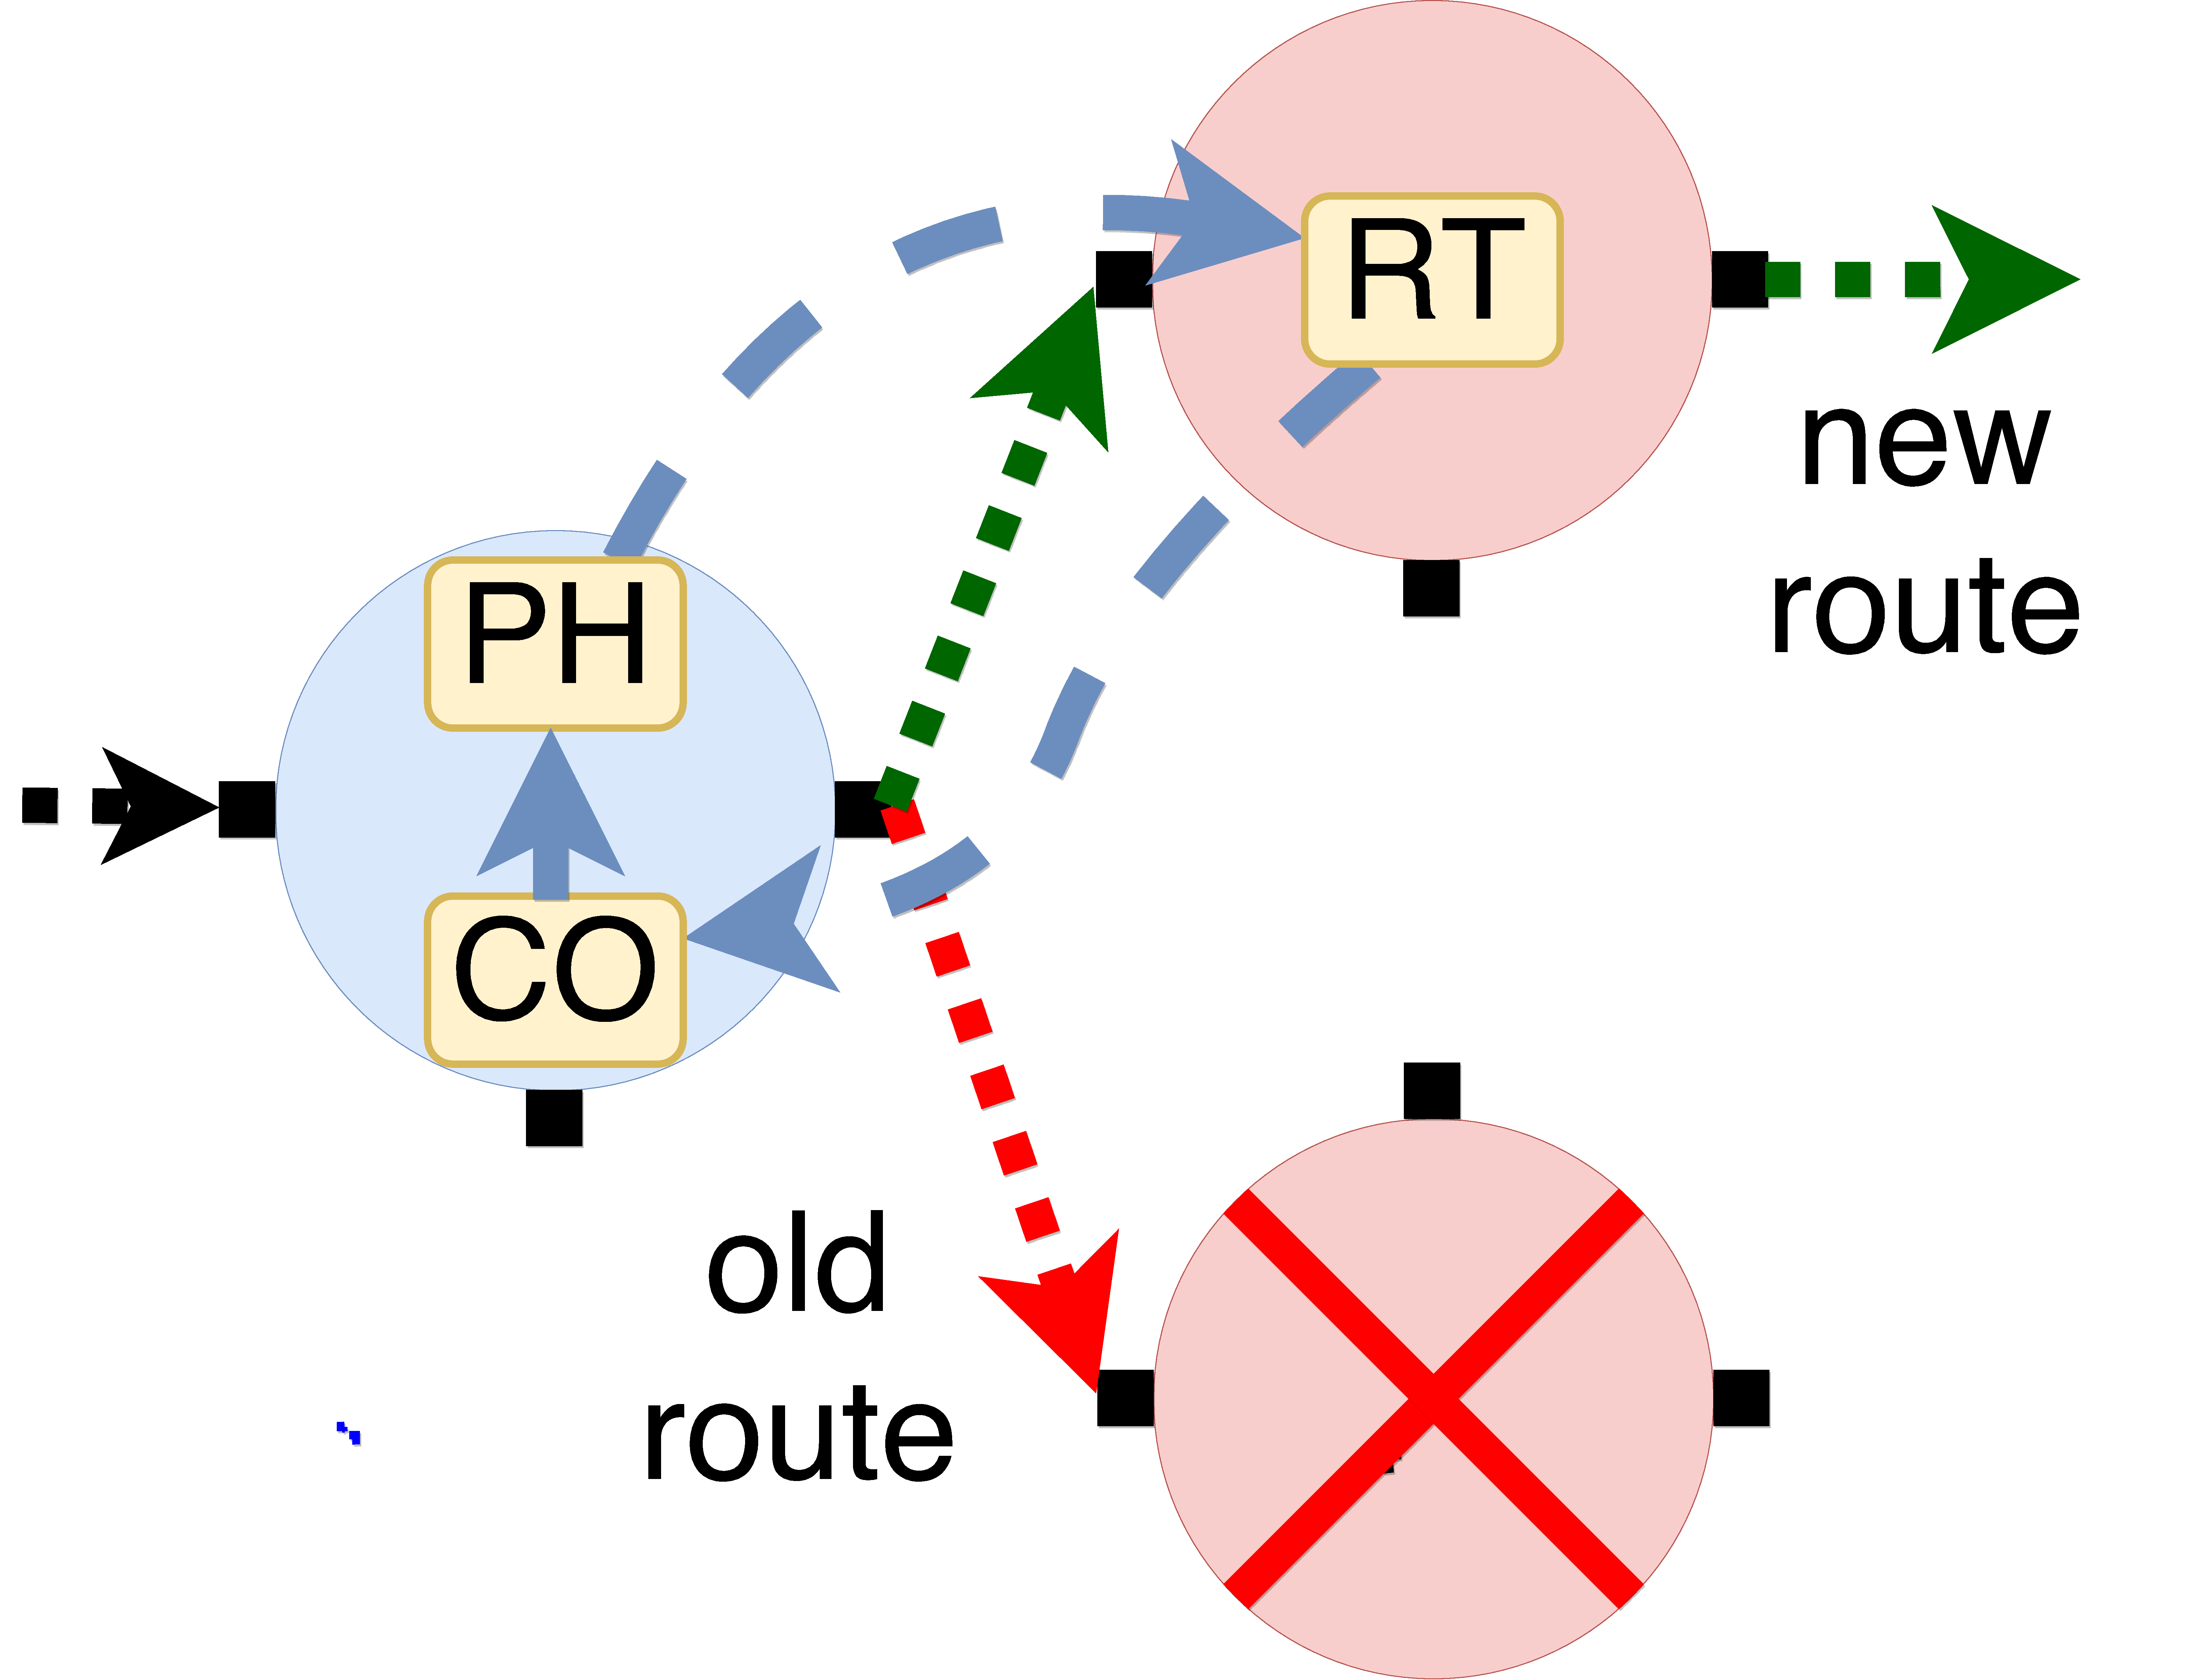
\includegraphics[width=0.66\columnwidth]{figure/nfactor-recover.pdf}
     \caption{Flow recover. The original runtime has failed.}\label{fig:recover}
    \end{subfigure}
 \caption{Flow replication that replicates the original actor running on the original runtime to replica runtime. (\textbf{RT}: Replication target actor. \textbf{RS}: Replication source actor. \textbf{CO}: Coordinator actor. \textbf{VS}: Virtual switch actor. \textbf{Dotted line}: Dataplane flow packets. \textbf{Dashed line}: Actor messages.)}
\label{fig:flow-rep}
\end{figure}

The biggest difference of the \nfactor's replication method and existing works such as \cite{sherry2015rollback} is that NFActor framework replicates individual flow, not NF. This replication strategy is transparent to the NF modules and improves the scalability and resource utilization rate of \nfactor. as flows could be directly replicated on another runtime, without the need for a dedicated backup server. In the mean time, this fine grained replication strategy provides a the same output-commit property as indicated in \cite{sherry2015rollback} with a desirable replication throughput and fast recovery time.

The detailed flow replication process is shown in figure \ref{fig:flow-rep}. When a flow actor is created, it acquires its replica runtime by querying a round-robin list. If the flow actor has a valid replica runtime, whenever it finishes processing the packet, it sends a remote message, containing the current flow state and the packet, to the coordinator actor on the replication target runtime. The coordinator actor on the replication target runtime creates a replica flow actor using the same flow-5-tuple as the original flow actor to handle all the replication messages. The replica flow actor saves the flow state and sends the packet out from the output port of the replica runtime. Similar with \cite{sherry2015rollback}, the receiver on the side of the output port of the replica runtime can only observe an output packet when the flow state has been replicated.

When a runtime fails, the controller sends recovery RPC requests \ref{} to all the replica runtime of the failed runtime. This RPC enables replica flow actor to send a request to the virtual switch actor, asking it to change the destination runtime to the replica runtime. When the response is received by the replica flow actor, the original flow is successfully restored on the replica runtime.
